\section{Systematic uncertainties}
\label{sect:sys}
Systematic uncertainties can affect the shape or normalization of the
backgrounds estimated from Monte Carlo (\ttbar, Z+jets, dibosons and Higgs decays), 
as well as the signal acceptance. 

\subsection{b-jet veto uncertainty due to mismodeling of ISR}
The jet activity in our signal is just due to Initial State Radiation(ISR). The ISR is not simulated properly in our signal, because it has been generated using \PYTHIA $6.4$ event generator and it just produces $2 \rightarrow 2$ scattering processes. Therefore the ISR jet momenta spectra and its multiplicity cannot be trusted. It is possible that an ISR jet is mistagged as a b-jet and results in vetoing the signal event after applying the b-veto cut. On the other side \MADGRAPH ~\cite{MADGRAPH} generator, which is a matrix element generator provides a better description of ISR jets by supporting $2 \rightarrow 4$ interactions. To measure the amount of uncertainty introduced by b-veto cut we can compare the efficiency of this cut in our generated signal and its value in a sample similar to our signal which has been generated by \MADGRAPH. 
The most similar MC sample to our signal from the production point of view is WW sample. The $m(\chione) = 100\,\GeV$ and $m(\PSGczDo) = 1\,\GeV$ point of the signal is chosen so that masses resembles the WW production mechanism. % It is followed the below recipe, originating from $fixME$.
%By applying and relaxing the b-veto cut it is obtained the yields of WW and signal and by the uncertainty is A:
We obtain the efficiency of b-veto for signal sample denoted as $E^{SUSY}_{b-veto}$ and also for WW sample denoted as $E^{WW}_{b-veto}$.
Comparing these 2 efficiencies this uncertainty can be estimated.

\begin{align}
E^{WW}_{b-veto} &= \frac{WW_{0b}}{WW_{all}} = \frac{88968.51}{93058.33} = 0.95\\ \nonumber
\end{align}
and the b-veto efficiency for the signal is:
\begin{align}
E^{SUSY}_{b-veto} &= \frac{SUSY_{0b}}{SUSY_{all}} = \frac{2041.88}{2206.07} = 0.92 \\ \nonumber
\end{align}
and we take:
\begin{align}
|\frac{E^{SUSY}_{b-veto}-E^{WW}_{b-veto}}{E^{WW}_{b-veto}}| &= 3 \% \\ \nonumber
\end{align}

\subsection{\texorpdfstring{Uncertainty due to $\mindphifour$ cut}{Uncertainty due to minDeltaPhiJMET cut}}
Another source of systematic uncertainty due to existence of ISR in signal events is the cut on $\mindphifour$ ($ > 1$) against QCD events. We use the same method as mentioned above to obtain the systematic uncertainty of applying this variable. But this time we use Higgs to $\tau \tau$ sample which mimics our signal most.

\begin{align}
E^{Higgs}_{\mindphifour} &= \frac{Higgs_{\mindphifour>1.0}}{Higgs_{all}} = \frac{89288.14}{180562.56} = 0.49 \\ \nonumber
\end{align}
and this efficiency for the signal is: 
\begin{align}
E^{SUSY}_{\mindphifour} &= \frac{SUSY_{\mindphifour>1.0}}{SUSY_{all}} = \frac{1020.33}{2206.07} = 0.46 \\ \nonumber
\end{align}
and we take:
\begin{align}
|\frac{E^{SUSY}_{\mindphifour}-E^{Higgs}_{\mindphifour}}{E^{Higgs}_{\mindphifour}}| &= 6 \% \\ \nonumber
\end{align}

\subsection{\texorpdfstring{$\ell$ and \Tau energy scale}{Energy scale}}
The systematic uncertainty due to muon energy scale is small enough to be ignored.

The electron energy is varied by $1\%$ ($2.5\%$) for electrons reconstructed in the barrel (endcap) region as recommended by EGAMMA POG\cite{eEnergyScale}. As this variation has small effects on electron $\pt$ related variables, its effect on final yields in \eTau channel has been found negligible.

The energy of \Tau's is scaled by $3\%$, following the recommendation of the Tau POG~\cite{TauPOG}. Variables like \MPT, \mttwo, \mindphifour and invariant mass which depend on \Tau $\pt$ are re-calculated.  Up and down uncertainties in the final yields are reported in table~\ref{Tab.tauEnergyScale}. 
\begin{center}
\begin{table}[!Hhtb]
\scriptsize{
\caption{Tau energy scale systematic effect on MC in different channels. The statistical uncertainty is also quoted to be able to guess the statistical contamination in the systematic values.}
\begin{tabular}{|c|c|c|c|c|c|c|}
\hline  
                            & ZX    & Higgs  & WW   & Top    & All MC & SUSY (380 , 1)%& Data%
 \\\hline 
$e\Tau$ channel            & $0.38\pm0.06^{+0.13}_{-0.08}$ & $0.06\pm0.02^{+0.0}_{-0.02}$  & $0.05\pm0.04^{+0.0}_{-0.0} $ &$0.02\pm0.02^{+0.02} _{-0.0}$  & $0.45\pm0.07^{+0.14}_{-0.03}$ & $2.14 \pm 0.10 ^{+0.07} _{-0.05} $ %& $3.0\pm1.73 ^{+0.0 \%} _{-33 \%}$
    \\\hline   
%^{+0.14}_{-0.03}
%W:$1.29\pm0.62^{+0.0}_{-0.0} $
$\mu\Tau$ channel      &  $0.28 \pm 0.05 ^{+0.14} _{-0.06} $      & $0.05\pm0.02^{+0.03}_{-0.0}$   & $0.34 \pm 0.14 ^{+0.37} _{-0.24} $        &  $0.0\pm0.0 ^{+0.67} _{-0.06} $   &    $0.66  \pm 0.15 ^{+0.34} _{-0.13} $      &  $2.16 \pm 0.11^{+0.09} _{-0.06} $      %& $5.0 ^{} _{} $     
\\\hline  
%$0.79 \pm 0.47^{+0.8} _{-0.35} $
$\tauTau$ \binone     &    $0.56 \pm 0.07 ^{+0.7} _{-0.09}$    & $0.17 \pm 0.04 ^{+0.05} _{-0.05}$       &  $0.02 \pm 0.02 ^{+0.0} _{-0.02}$        &   $0.0 \pm 0.0 ^{+0.0 } _{-0.0 }$        &    $0.75 \pm 0.08 ^{+0.21} _{-0.19}$     & $4.10 \pm 0.38^{+0.05} _{-0.03} $    %& $1.0 \pm1.0 ^{+0.0 \%} _{-0.0 \%}$
\\\hline
%$0.0 \pm 0.0 ^{+0.0} _{-0.0}$
$\tauTau$ \bintwo    &     $0.81 \pm 0.56 ^{+0.39} _{-0.7}$     &   $0.07 \pm0.02 ^{+0.02} _{-0.03}$      &     $0.15 \pm 0.07 ^{+0.0} _{-0.02}$     &   $0.53 \pm 0.53 ^{+0.0} _{-0.0}$   &      $1.48 \pm 0.77 ^ {+0.49} _{-0.28}$     &     $1.10 \pm 0.07 ^{+0.04} _{-0.02}$   %&  $2.0 \pm 1.41 ^{} _{}$   
 \\\hline
%$0.43 \pm 0.4 ^{+0.0} _{-0.0 }$
\end{tabular} 
\label{Tab.tauEnergyScale}
}
\end{table}     
\end{center}
The big value of the \Tau energy scale uncertainty is dominated by the lack of the statistics. In signal samples which have enough statistics the uncertainty decreases. 
In some cases which the statistical uncertainty had a large value comparing to systematic uncertainty, 
we relaxed some \Tau \pt  independent variables to obtain more statistics. 
In another approach, the \pt related cuts are applied one by one and uncertainty of each cut is calculated independently. 
Finally, all individual uncertainties are taken to be independent and added in quadrature. The final uncertainties due to
tau energy scale vary in the range of 10-15\% and 2-15\% in different signal regions for backgrounds and signals, respectively.
%Eskandari's presentation 8 April 2015

%So the maximum uncertainty due to \Tau energy scale in MC driven backgrounds and signal is set to $~10\%$.
%In order to calculate systematic uncertainties for signal, we used 3 signal points which are ($m(\chione) = 180\,\GeV$, $m(\PSGczDo) = 60\,\GeV$), (240, 40) and (380, 1) representing low, moderate and high delta mass respectively. 
%The $10\%$ effect of this uncertainty for all signal points in different channels is a conservative value that covers the whole plain and all channels.


\subsection{Monte Carlo  statistics} 
The statistics in the simulated Monte Carlo samples are also a
  source of the  uncertainties. % which are 20\% for the background processes and 10\% for the signal events.
This uncertainty varies for signal points between 3\% and 15\% and for the backgrounds between 13\% and 70\%.

\subsection{b-jet ID}
The uncertainty due to the b-tag scale factor on the signal and background events is taken into account by varying the scale factors within their 
uncertainty. It is found that for signal, there is an uncertainty of about $8\%$. For almost all of the backgrounds except for backgrounds including Top, an uncertainty around 1\% is found. For Top backgrounds, the uncertainty is about 4\%. Therefor, for background events at most a 4\% uncertainty due to the b-veto cut is assigned. 
 
\subsection{Lepton trigger, identification and isolation efficiency}
The uncertainties in electron and muon triggers, identification and isolation efficiencies are $2\%$ for electrons and muons ~\cite{CMS_AN_2013-171}. The uncertainty in the \Tau identification efficiency amounts to $6\%$ ~\cite{CMS_AN_2013-171}
The uncertainty in the efficiency of the hadronic tau leg of the $e\Tau$ and $\mu\Tau$ ($\tauTau$) trigger amounts to $3.0\%$ ($4.5\%$ per leg).

\subsection{PDF}
The signal acceptance changes due to PDF uncertainties is expected to be small. We take this uncertainty from ~\cite{CMS_AN_2012-248}, where the signal has been produced through electroweak process like our signal. The amount of this uncertainty is around $2\%$.

%The effect of PDF on cross section is considered using $CTEQ66$ and $MSTW2008nlo90cl$ for PDF and it is shown for some generic SUSY points in Table.~\ref{Tab.PDF}.
%\begin{table}[!Hhtb]
%\begin{center}
%\caption{Cross section systematic uncertainty due to different PDF.}
%\begin{tabular}{|c|c|c|}
%\hline
%                                    &$\sigma (fb) \_ CTEQ66$          & $\frac{\sigma \_ CTEQ66 - \sigma \_ MSTW2008}{\sigma \_ CTEQ66}$  \\\hline 
%m(\chione) = 100 GeV                &$5823.40^{+0.0 \% + 3.4 \%}_{-0.6 \% - 3.2 \%}$         & 3 \%         \\\hline   
%m(\chione) = 200 GeV                &$379.24^{+0.4 \% + 4.5 \%}_{-0.4 \% - 4.4 \%}$          & 6 \%        \\\hline  
%m(\chione) = 300 GeV                &$67.51^{+0.2 \% + 5.9 \%}_{-0.2 \% - 5.1 \%}$           & 7 \%        \\\hline
%m(\chione) = 400 GeV                &$17.51.40^{+0.0 \% + 6.8 \%}_{-0.3 \% - 6.3 \%}$        & 8 \%        \\\hline
%m(\chione) = 500 GeV                &$5.53^{+0.0 \% + 8.1 \%}_{-0.9 \% - 7.0 \%}$            & 12 \%        \\\hline
%\end{tabular} 
%\label{Tab.PDF}
%\end{center}
%\end{table}     

\subsection{Luminosity}                                                                                                                                                           
The uncertainty in the luminosity  is $2.6\%$ for $2012$ data ~\cite{LUMI}.                                                                                                       
This affects mainly the  normalization of the signal Monte Carlo samples, because for the backgrounds  either  the data-driven methods are used or
the normalization is found from data.

\subsection{Pile-up}
The minimum bias cross section is varied $5 \%$ up and down following the standard recipe of ~\cite{PU_SYS}. It is found to introduce $~4 \%$ systematic for all channels.    

\subsection{\texorpdfstring{\MPT}{MET}}
The main backgrounds come from data driven or MC validated against data. \MPT uncertainties can be important for signal only. Our signal is produced through a SUSY EWK production and does not include jets directly but it is expected to feature four invisible particles as genuine missing energy. Therefore it should not be affected by jet calibrations. Apart from jets, lepton and tau energy scales and their effects on \MPT have been already taken into account. There is just unclustered energy left which based on results in ~\cite{CMS_AN_2014-099} this item's effect on \MPT is small enough to be ignored.



\subsection{\texorpdfstring{Inefficiency due to a bug in \Tau trigger}{Inefficiency due to a bug in tau trigger}}
To consider the effect of a known trigger bug in $\tauTau$ channel~\cite{CMS_AN_2014-074}, the $\pt$ 
distribution of the leading \Tau in \binone for the signal SMS point corresponding to (380,1) is shown (in black) in figure~\ref{fig:tauPt}.
\begin{figure}[!Hhtb]
\centering
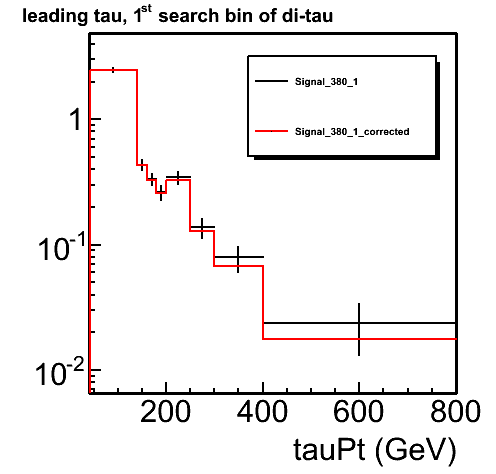
\includegraphics[angle=0,scale=0.35]{TauTauFigs/leadingTauPt.png}
\caption{The $\pt$ distribution of the leading \Tau in \binone of the $\tauTau$ channel. Also shown is the modified $\pt$ distribution after correction for the trigger bug.}
\label{fig:tauPt}
\end{figure}

 The choice of this signal point is because of the fact that this SMS point can provide the maximum efficiency of 
having \Tau with $\pt$s above 140 \GeV.  In the same plot, the modified pt-distribution is shown in red, 
which is obtained as follows. Based on figure~35 of the same reference, a correction factor is taken and 
multiplied bin-by-bin to the black histogram (for the bins above 140 GeV). The difference in integral
of the two histograms is of the order of ~1.5\% (original integral equals 4.10, while the modified integral is equal to 4.04).
Due to smallness of this effect comparing to other systematic, it is ignored and no correction is applied. 


\subsection{\texorpdfstring{\Tau efficiency in fast simulation}{Tau efficiency in fast simulation}}
The fast simulation shows some differences with the full simulation, especially in track reconstruction. It can affect the \Tau isolation.
To evaluate the effect of this inefficiency, the \Tau isolation/identification efficiency  is compared in the fast and full simulation.
Figure \ref{fig:TauEffFastFull} (left)
\begin{figure}[!Hhtb]
\centering
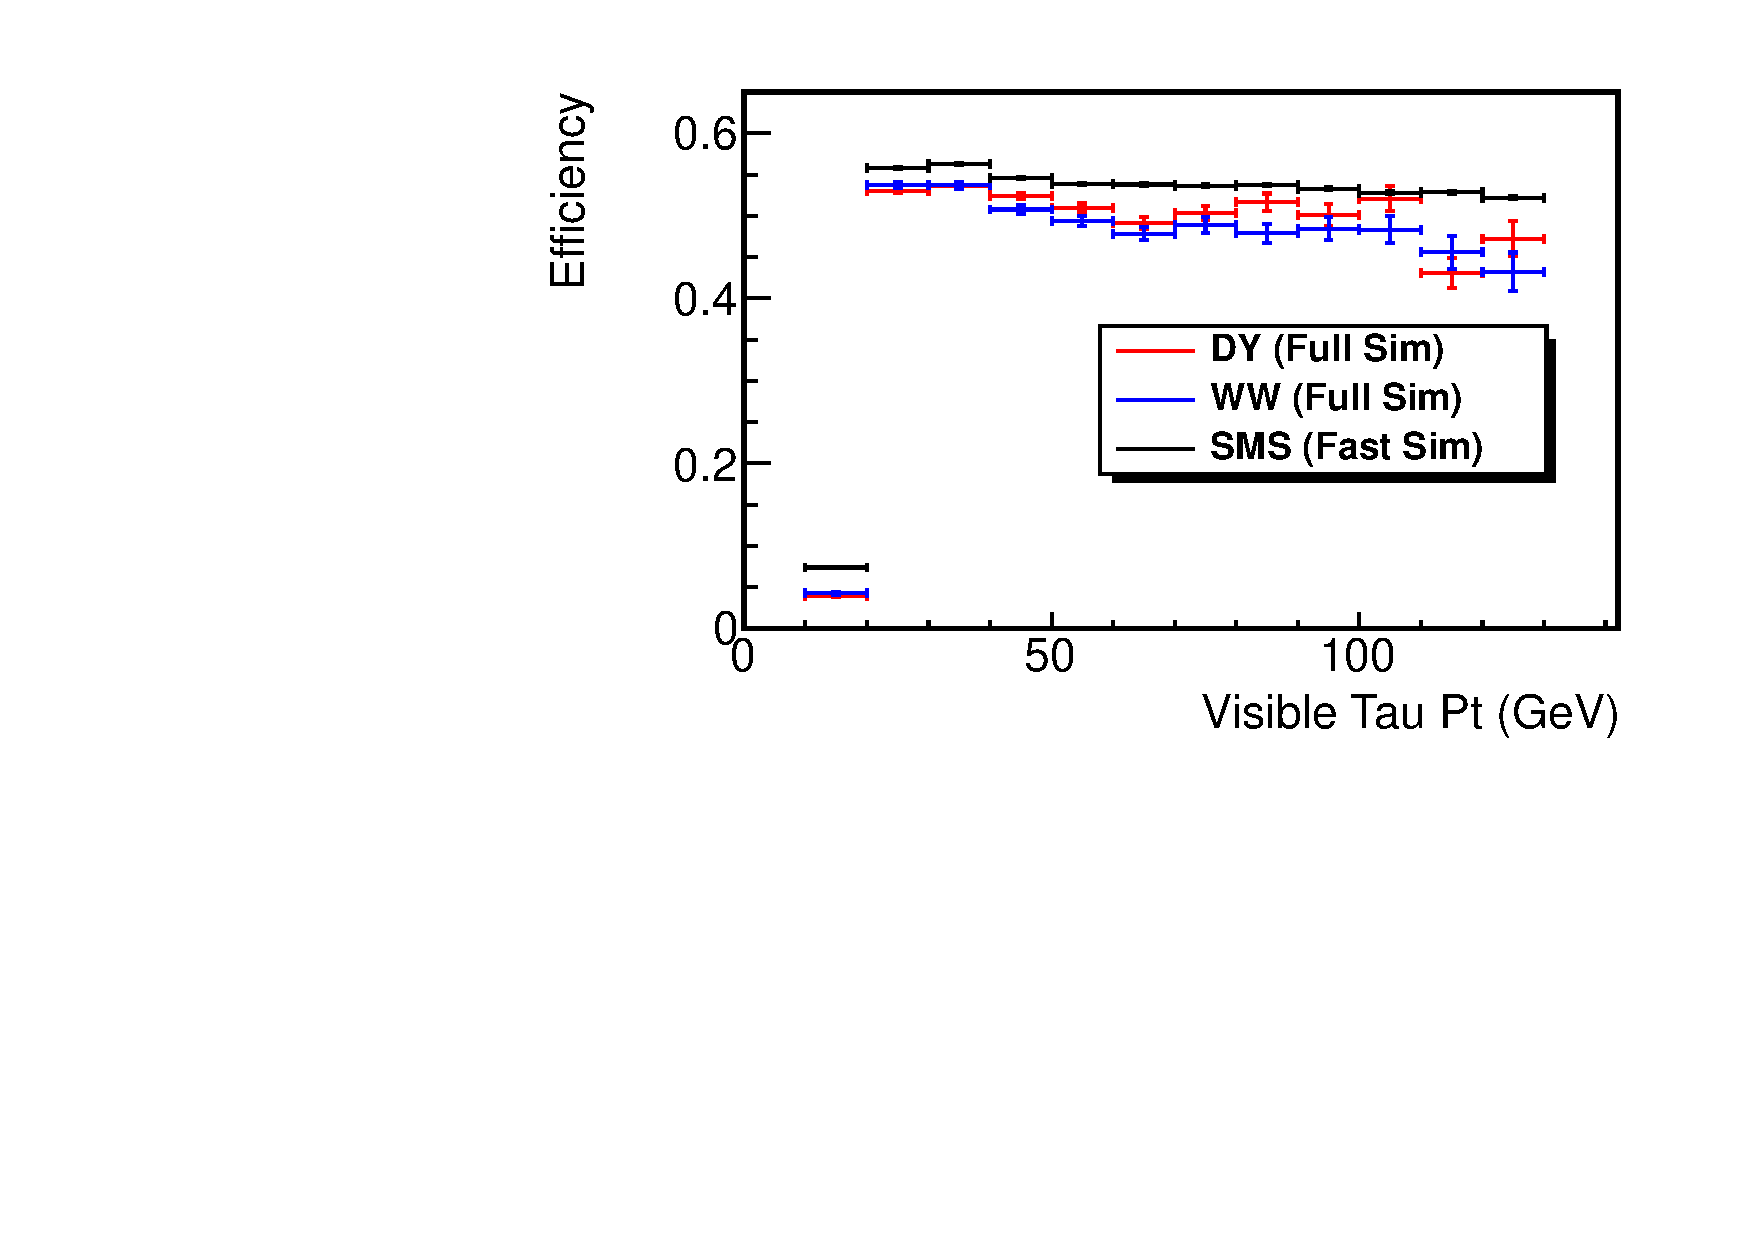
\includegraphics[angle=0,scale=0.35]{SystematicFigs/TauEff_lepTau.pdf}
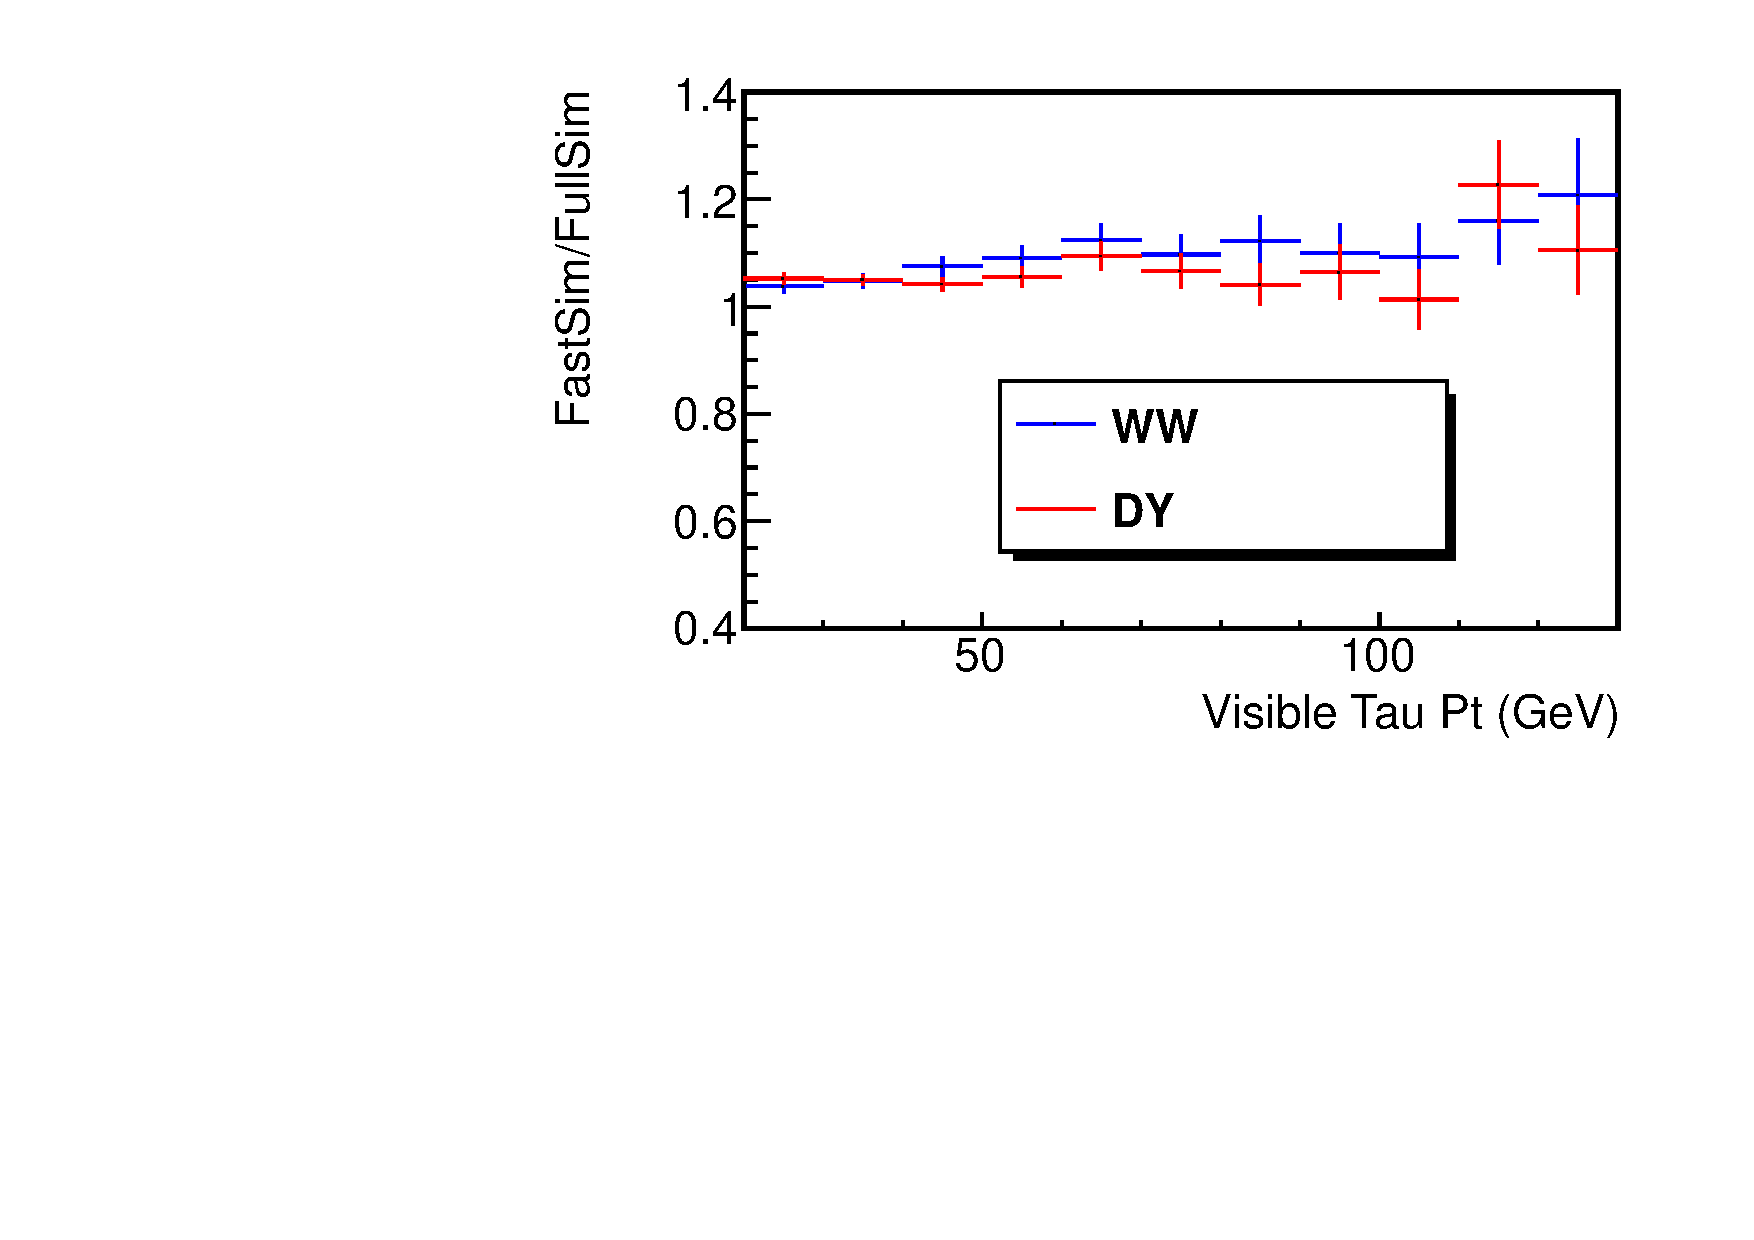
\includegraphics[angle=0,scale=0.35]{SystematicFigs/TauEff_lepTau_ratio.pdf}
\caption{Comparison of the \Tau efficiency in the full and fast simulation (left). The ratio of the efficiencies in the fast and full simulation. (right)}
\label{fig:TauEffFastFull}
\end{figure}
compares the \Tau efficiency in WWjets and DYjets which are full simulation with signal which is fast simulation. In 
both cases, only \Tau in \leptonTau channels are considered. In 
\ref{fig:TauEffFastFull} (right), the ratio of the efficiency of the fast simulation to full simulation is shown. 
The main source of the difference, is the difference between the additional event activities in the samples, so we assign 5\% systematic uncertainty per \Tau leg.

\subsection{Low rate backgrounds} For some backgrounds like \ttbar, dibosons and Higgs decays, the remaining 
events from the simulation are very small. A 50\% uncertainty is considered for these backgrounds to account for the theoretical uncertainty of the
cross section calculation as well as the shape mismodeling.

\subsection{Summary}
The summary of all systematic uncertainties for different channels is reported in Table.~\ref{Tab.SYS}. The main source of the systematic uncertainty in all channels and samples is the \Tau energy scale.  
The systematic uncertainties that can alter the shapes are added in quadrature and 
treated correlated when two signal regions of \tauTau channel are combined. Other systematic uncertainties of these two 
channels and all of the systematic uncertainties of \leptonTau channels are treated uncorrelated.

%We add all systematic uncertainties in quadrature and assign 
% 20\% and 25\% relative uncertainties in the signal
%acceptance for the \leptonTau and \tauTau channels, respectively. For the Monte Carlo background predictions, the values are 
%25\% and 28\%, respectively. The relative uncertainty of the less important backgrounds is 50\% for all channels.

\begin{table}[!htb]
\begin{center}
\caption{Summary of systematic uncertainties that affect the signal event selection efficiency and the background normalization and their shape. The sources that alter
the shape are indicated by (*) next to their names. The shape-altering sources are considered correlated between two signal regions of \tauTau in the final statistical combination.}
\small{
\begin{tabular}{|l|ccc|ccc|}
\hline\hline
                              &\multicolumn{3}{c|}{Background}         &\multicolumn{3}{c|}{Signal}\\\hline
                              &            & \tauTau & \tauTau         &            & \tauTau & \tauTau\\
Systematic uncertainty source & \leptonTau & \binone &  \bintwo        & \leptonTau & \binone &  \bintwo        \\
\hline\hline
%*\Tau energy scale&\multicolumn{3}{c|}{10} &\multicolumn{3}{c|}{10} \\\hline
\Tau energy scale (*)&10\% &\multicolumn{2}{c|}{15\%}  & 2-12\% &\multicolumn{2}{c|}{3-15\%} \\\hline 
\Tau id efficiency& 6\% &\multicolumn{2}{c|}{12\%} & 6\% &\multicolumn{2}{c|}{12\%}  \\\hline
\Tau trigger efficiency& 3\%&\multicolumn{2}{c|}{9\%}& 3\%&\multicolumn{2}{c|}{9\%}  \\\hline
Lepton trigger, id, iso efficiency& 2\% & \multicolumn{2}{c|}{-} & 2\% &  \multicolumn{2}{c|}{-} \\\hline
\MPT (*)&\multicolumn{3}{c|}{5\%} &\multicolumn{3}{c|}{5\%} \\\hline
b-tagged jets veto & 4\% & - & 4\% &  8\% & - & 8\% \\\hline
Pile-up&\multicolumn{3}{c|}{4\%} &\multicolumn{3}{c|}{4\%} \\\hline
Fast/Full \Tau id efficiency &\multicolumn{3}{c|}{-}& 5\% & \multicolumn{2}{c|}{10\%}\\\hline
ISR (*)&\multicolumn{3}{c|}{-}&\multicolumn{3}{c|}{3\%} \\\hline
\mindphifour&\multicolumn{3}{c|}{-}&\multicolumn{3}{c|}{6\%} \\\hline
PDF (*)&\multicolumn{3}{c|}{-}&\multicolumn{3}{c|}{2\%} \\\hline
Luminosity       &\multicolumn{3}{c|}{-} & \multicolumn{3}{c|}{2.6\%}\\\hline
Total shape-altering Sys. & 11\% & 16\% & 16\% & 6-13\% &\multicolumn{2}{c|}{7-16\%} \\\hline
Total non-shape-altering Sys. & 9\% & 16\% & 16\% & 14\% &20\%& 21\% \\\hline
Total Systematic&  14\% & 22\%  & 22\%& 15-19\% & 21-25\%  & 22-26\%\\\hline
Monte Carlo Statistic & 22\% & 13\% & 70\% & \multicolumn{3}{c|}{3-15\%} \\\hline
Total& 26\% & 26\%  & 73\%& 15-24\% & 21-29\%  & 22-30\%\\\hline
Low rate backgrounds &\multicolumn{3}{c|}{50\%}&\multicolumn{3}{c|}{-}\\\hline
\hline
\end{tabular}
}
\label{Tab.SYS}
\end{center}
\end{table}

